% !TEX root = ./main.tex
\documentclass[a4paper]{article}
% Course language: use [english] or [german].
\usepackage[german]{ajnotes}
\title{Mathematik I — Day 1 Summen und Prodzeichen}
\begin{document}
    \maketitle
    % Attach the given problem sheet: drop it in this folder as sheet.pdf and
    % un-comment the next line (pdfpages is already loaded by the preamble).
    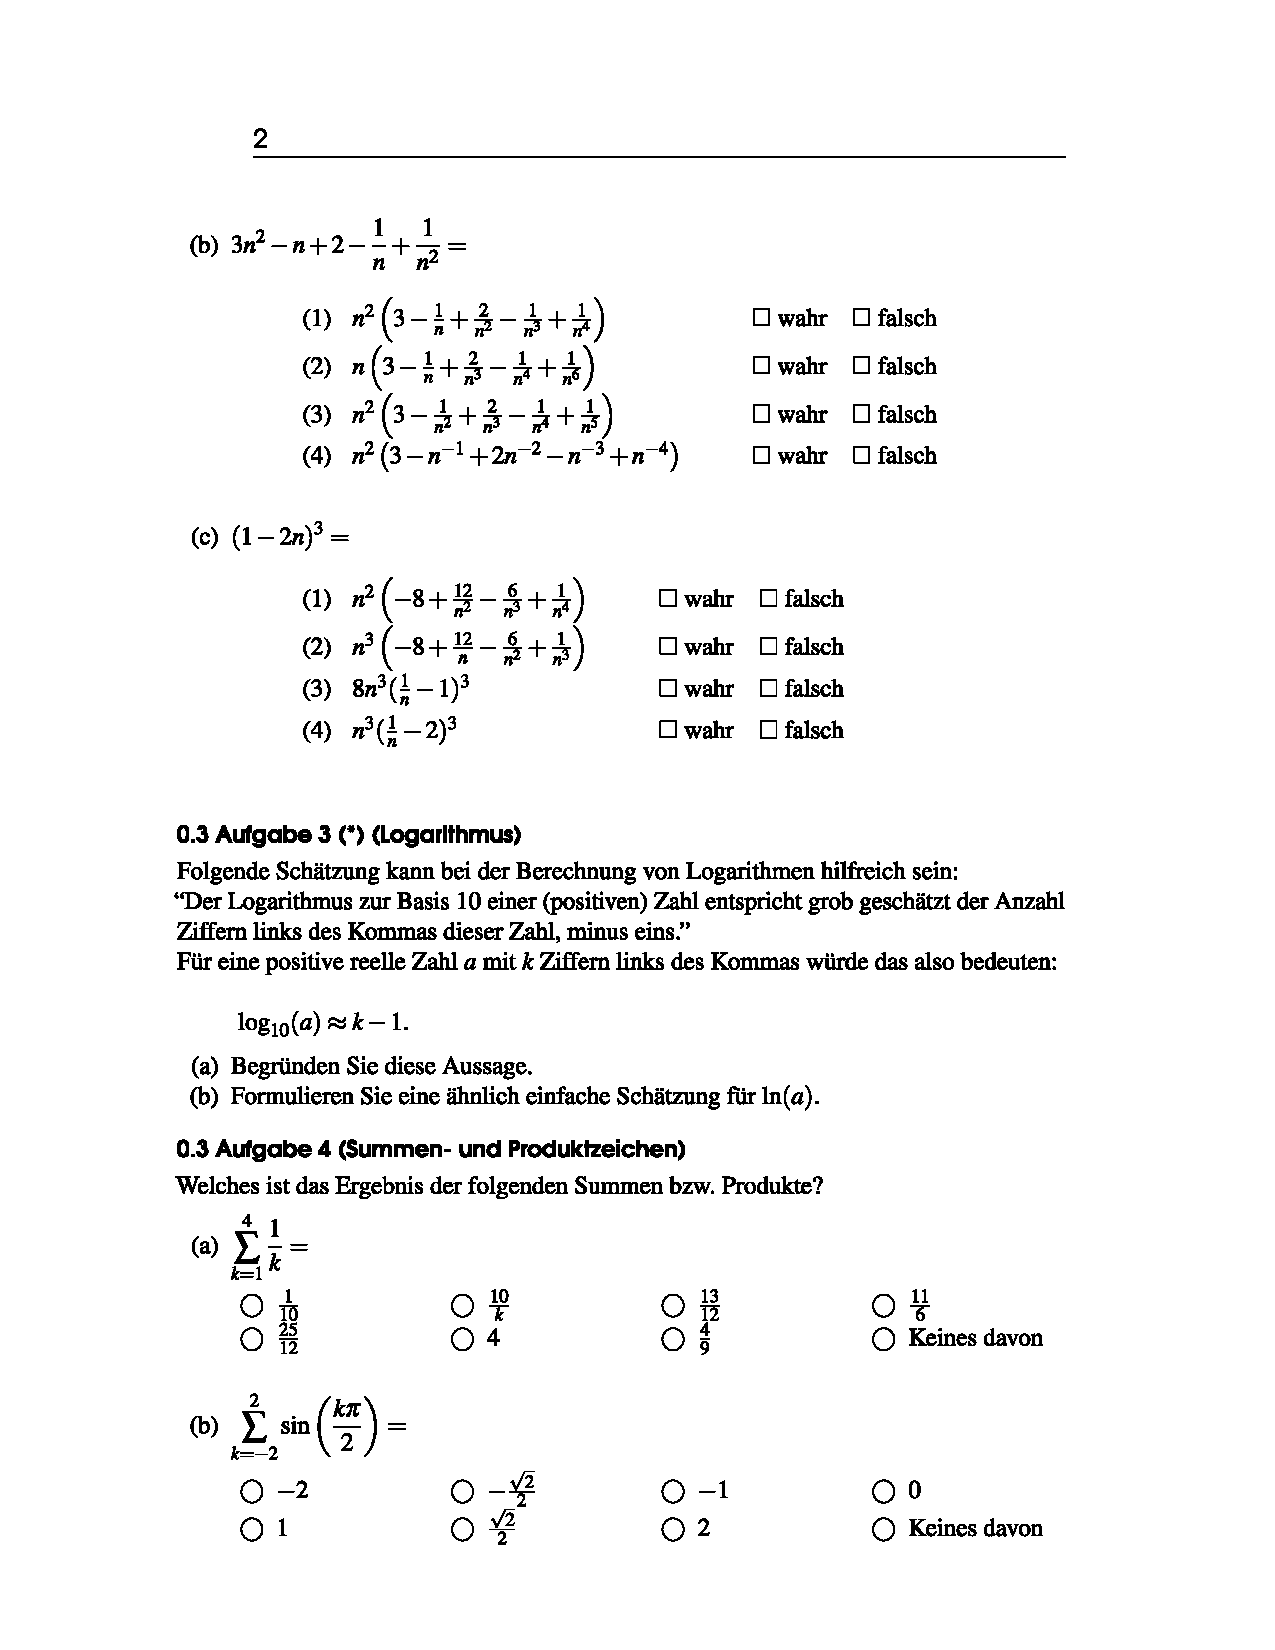
\includepdf[pages=-]{sheet.pdf}
    \exercise{1}
    
    \subexercise{a}

\end{document}
